\documentclass[mathserif]{beamer}

\usepackage{beamerthemesplit} % // Activate for custom appearance

\usepackage{xeCJK}
\usepackage{graphbox}
\usepackage{subcaption}
\usepackage{tikz}
\usepackage{pgfplots}
\usepackage{listings}
\usepackage{makecell}
\usepackage{metalogo}
\usepackage{mflogo}
\usepackage{qrcode}
\usepackage{array}
\usepackage{svg}

\definecolor{nthu}{HTML}{7F1084}
\definecolor{secondary}{HTML}{910A17}
\definecolor{accent}{HTML}{410A91}

\usetheme{Warsaw}
\usecolortheme[named=nthu]{structure}
\useinnertheme{rounded}
\useoutertheme{infolines}
%\usefonttheme[onlymath]{serif}

\setbeamercolor{alerted text}{fg=secondary}
\setbeamercolor{example text}{fg=accent}

\xeCJKsetup{CJKglue=\hspace{0pt plus .12 \baselineskip }}
\xeCJKsetup{RubberPunctSkip=false}
\xeCJKsetup{PunctStyle=plain}
\xeCJKsetup{CheckSingle=true}
\XeTeXlinebreaklocale "zh"
\XeTeXlinebreakskip = 0pt plus 2pt

\setCJKmainfont{Apple LiSung}
\setCJKsansfont{Apple LiGothic}
%\setCJKmonofont{Noto Sans Mono CJK TC}

\lstset{
	basicstyle=\ttfamily,
	breaklines=true
}

\title[使用 Markdown 和 \LaTeX\ 成為筆記大師]{CSST 2022}
\subtitle{使用 Markdown 和 \LaTeX\ 成為筆記大師}
\author[nevikw39]{nevikw39 a.k.a. 翁君牧}
\institute[CSST]{清華資工系學會教學股 \and CSST 2022 籌備團隊}
\date{\today}
%\titlegraphic{\includegraphics[width=1.5cm]{nthu}}

\graphicspath{ {./figures} }

\AtBeginSection{
	\frame
	{
%		\frametitle{Outline}
		\sectionpage
		\tableofcontents[
			sectionstyle=show/shaded,
            subsectionstyle=show/show/hide,
            subsubsectionstyle=show/show/show/hide
        ]
	}
}

\begin{document}

\frame{\titlepage}

\frame{\tableofcontents}

\begin{frame}{Quick Links}

\begin{columns}

\column{.5\linewidth}

\color{nthu}
\url{https://github.com/nevikw39/CSST2022}

\column{.5\linewidth}

\qrcode[height=\linewidth]{https://github.com/nevikw39/CSST2022}

\end{columns}

\end{frame}

\begin{frame}{\ttfamily \$whoami}{nevikw39}

\begin{columns}

\column{.5\linewidth}

In case somebody is of interest, please refer to previous slides.

\column{.5\linewidth}


\includegraphics[width=\linewidth]{nevikw39}

\end{columns}

\end{frame}

\section{Markdown}

\begin{frame}{Where could Markdown be used or seen?}{Why Markdown?}


\includegraphics[width=.3\linewidth]{dc}

\includegraphics[width=.3\linewidth]{tg}

\includegraphics[width=.3\linewidth]{slack}

\includegraphics[width=.3\linewidth]{gh}

\includegraphics[width=.3\linewidth]{so}

\includegraphics[width=.3\linewidth]{rd}

\end{frame}

\begin{frame}{What's Markdown?}{}

\begin{block}{Markup Languages}
Describes some plain text files in a certain fashion that are easily read, written and transferred.

\begin{description}
\item[Human friendly] HTML, \TeX, Markdown, etc.
\item[Machine friendly] XML, JSON, YAML, TOML, ...
\end{description}
\end{block}

Markdown is a lightweight markup language for human's purpose.

\end{frame}

\begin{frame}{How to use Markdown?}{}

\begin{description}
\item[Ad-hoc softwares] Typora, Notion, ...
\item[Ordinary editors] VS Code, Sublime, Atom, Notepad++, ...
\item[Online services] HackND, GitHub Gist, ...
\end{description}

\end{frame}

\subsection{Basic Syntax}

\frame{Demo Time!}

\subsection{HackMD Extensions}

\frame{Demo Time!}

\section{\LaTeX}

\begin{frame}{Where could \TeX/\LaTeX\ be used or seen?}{Why \TeX/\LaTeX?}

\begin{tabular}{c|c}

\includegraphics[width=.45\linewidth,page=5,trim=1.5in 7.5in 1.5in 1.875in,clip]{Solution-of-Calculus} & 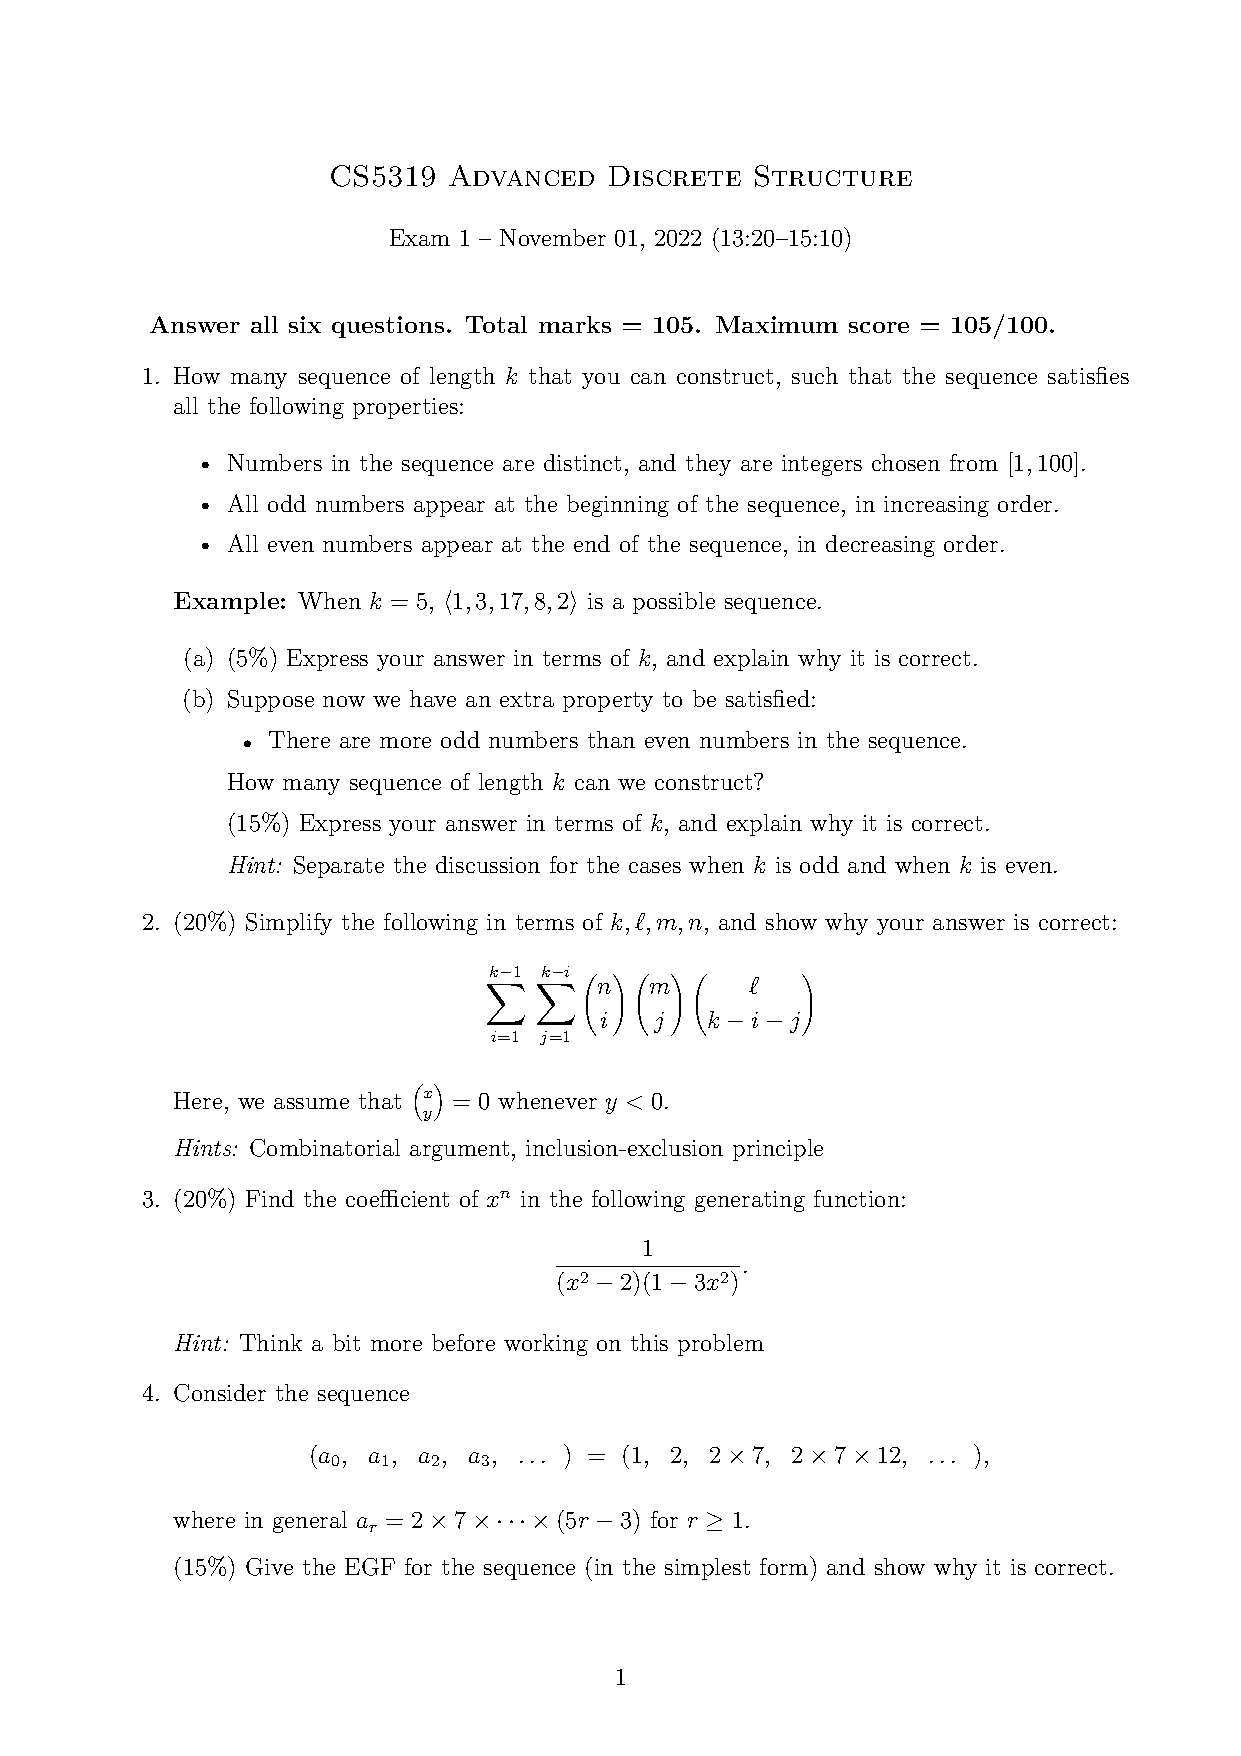
\includegraphics[width=.45\linewidth,page=1,trim=.87in 2.5in 1.69in 7.875in,clip]{exam1-2022}\\\hline
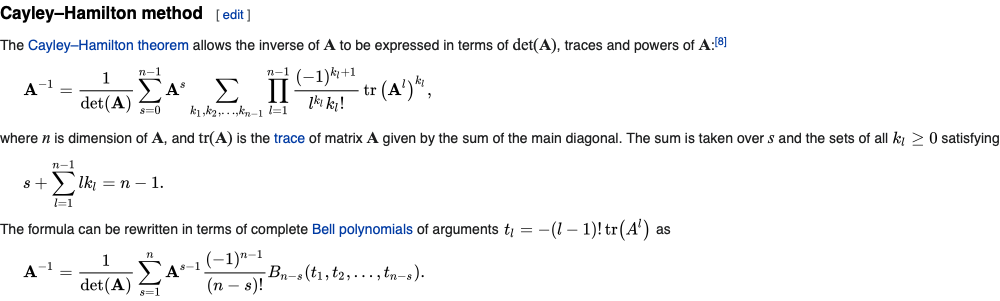
\includegraphics[width=.45\linewidth,align=c]{linalg} & 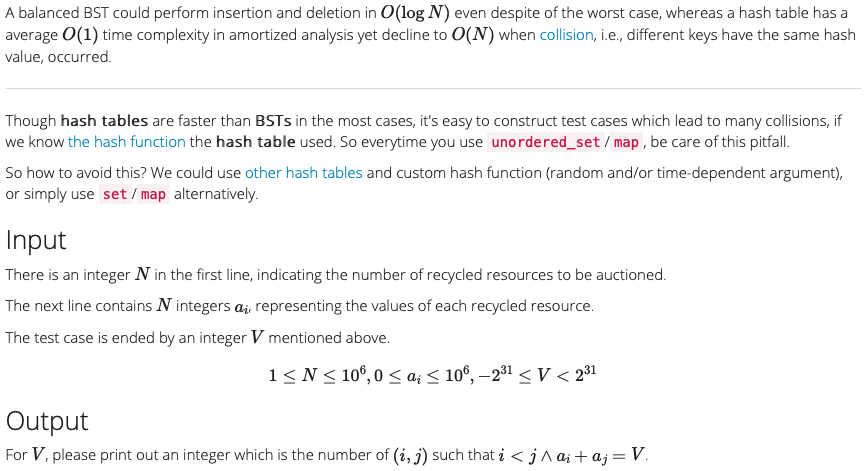
\includegraphics[width=.45\linewidth,align=c]{oj}
\end{tabular}

\end{frame}

\begin{frame}{Introduction}{}

\begin{itemize}
\item \TeX\ is a free, professional typesetting software widely used in academia
\item Developed by Knuth, D. E. for his chef d'\oe uvre \textit{The Art of Computer Programming}
\item Nowadays there are quite a few \TeX\ derivations, such as \textrm{\LaTeX}, \textrm{\XeTeX}, \textrm{\LuaTeX}, \textrm{\XeLaTeX}, \textrm{\LuaLaTeX}, \textrm{Con\TeX t}...
\item Many projects and solution port the core \TeX\ feature --- math typesetting --- onto webpages, other document softwares, etc.
\end{itemize}

\end{frame}

\begin{frame}{Characteristics}{}

\begin{itemize}
\item Classic yet chic \textrm{Computer Modern} font family built with \MF
\item Detailed and elaborate font settings, such as \textit{kerning}, \textit{ligature}, \textit{glyph variant}, ...
\item Expertise in displaying mathematical formulae (enhanced even further on top of \AmS-\TeX)
\item Apt and elegant algorithms for \textit{spacings}, \textit{breaks}, \textit{justification}, \textit{hyphenation}...
\item Rich support from vigorous community; that is, there are plenty of packages (e.g., to draw diagrams, etc.) and it's easy to seek answers online
\end{itemize}

\end{frame}

\begin{frame}{Distribution Installation \& Online Environment}{}

\begin{block}{\TeX\ Distributions}
One could install suitable \TeX\ Distribution for his OS, e.g. \TeX\ Live for Linux, Mac\TeX\ (derived from \TeX\ Live) for macOS or Mik\TeX\ for Windows.

Nevertheless, \TeX\ requires large disk space -- $\approx7.2$ G for \TeX\ Live 2021 by Mac\TeX--, and the install process is a bit tricky.
\end{block}

In addition, \textbf{Overleaf} is an online \LaTeX\ environment that supports partial-WYSIWYG, in-time collaboration.

Account with NTHU email address could gain premium \textbf{Overleaf} access for free!

\end{frame}

\subsection{Mathematical Formulae}

\begin{frame}[fragile]{Two modes for math expressions}{}

\begin{block}{Inline mode}
Enclose math commands in \verb|\( \)| or \texttt{\$} like \verb|$\hat{F}(x)=(1-5x)^\frac{-2}{5}$| to make the expression be within context like $\hat{F}(x)=(1-5x)^\frac{-2}{5}$.
\end{block}

\begin{block}{Display mode}
Enclose math commands in \verb|\[ \]| or two consecutive \texttt{\$}s like \verb|$$\hat{F}(x)=(1-5x)^\frac{-2}{5}$$| to make the expression stand out of context like: $$\hat{F}(x)=(1-5x)^\frac{-2}{5}$$.
\end{block}

\end{frame}

\begin{frame}[fragile]{Examples}{Limit}
\begin{alertblock}{Sources}
\small
\begin{lstlisting}[language=TeX]
$$\lim_{x\to c}f(x)=L\iff\forall\varepsilon>0,\exists\delta>0,0<|x-c|<\delta\implies|f(x)-L|<\varepsilon$$
\end{lstlisting}
\end{alertblock}
\begin{exampleblock}{Results}
$$\lim_{x\to c}f(x)=L\iff\forall\varepsilon>0,\exists\delta>0,0<|x-c|<\delta\implies|f(x)-L|<\varepsilon$$
\end{exampleblock}
\end{frame}

\begin{frame}[fragile]{Examples}{Integral}
\begin{alertblock}{Sources}
\begin{lstlisting}[language=TeX]
$$\int_a^bf(x)dx=\lim_{n\to\infty}\sum_{i=1}^n\frac{b-a}{n}f(a+\frac{b-a}{n}i)$$
\end{lstlisting}
\end{alertblock}
\begin{exampleblock}{Results}
$$\int_a^bf(x)dx=\lim_{n\to\infty}\sum_{i=1}^n\frac{b-a}{n}f(a+\frac{b-a}{n}i)$$
\end{exampleblock}
\end{frame}

\begin{frame}[fragile]{Examples}{}
\begin{alertblock}{Sources}
\begin{lstlisting}[language=TeX]
$$x=\frac{-b\pm\sqrt{b^2-4ac}}{2a}$$
\end{lstlisting}
\end{alertblock}
\begin{exampleblock}{Results}
$$x=\frac{-b\pm\sqrt{b^2-4ac}}{2a}$$
\end{exampleblock}
\end{frame}

\begin{frame}[fragile]{Examples}{Stirling's formula}
\begin{alertblock}{Sources}
\begin{lstlisting}[language=TeX]
$$n!\approx\sqrt{2\pi n}(\frac{n}{e})^n$$
\end{lstlisting}
\end{alertblock}
\begin{exampleblock}{Results}
$$n!\approx\sqrt{2\pi n}(\frac{n}{e})^n$$
\end{exampleblock}
\end{frame}

\begin{frame}[fragile]{Examples}{Generalized Binomial Theorem}
\begin{alertblock}{Sources}
\begin{lstlisting}[language=TeX]
$$(1+x)^r=\sum_{k=0}^\infty\binom{r}{k}x^k$$
\end{lstlisting}
\end{alertblock}
\begin{exampleblock}{Results}
$$(1+x)^r=\sum_{k=0}^\infty\binom{r}{k}x^k$$
\end{exampleblock}
\end{frame}

\begin{frame}[fragile]{Examples}{Master Theorem}
\begin{alertblock}{Sources}
\begin{lstlisting}[language=TeX]
$$T(n)=aT(\frac{n}{b})+O(n^d)=\left\{\begin{array}{ll} O(n^d), & d>\log_b a \\ O(n^d\log n), & d=\log_b a \\ O(n^{\log_b a}),&d<\log_b a \end{array}\right.$$
\end{lstlisting}
\end{alertblock}
\begin{exampleblock}{Results}
$$T(n) = aT(\frac{n}{b}) + O(n^d) = \left\{\begin{array}{ll}O(n^d), & d > \log_b a\\O(n^d\log n), & d =\log_b a\\O(n^{\log_b a}), & d < \log_b a\end{array}\right.$$
\end{exampleblock}
\end{frame}

\begin{frame}[fragile]{Examples}{Block Matrix LDU Decomposition}
\begin{alertblock}{Sources}
\begin{lstlisting}[language=TeX]
\small
$$\begin{pmatrix}A_{0,0}&A_{0,1}\\A_{1,0}&A_{1,1}\end{pmatrix}=\begin{pmatrix}I&O\\A_{1,0}A_{0,0}^{-1}&I\end{pmatrix}\begin{pmatrix}A_{0,0}&O\\O&A_{1,1}-A_{1,0}A_{0,0}^{-1}A_{0,1}\end{pmatrix}\begin{pmatrix}I&A_{0,0}^{-1}A_{0,1}\\O&I\end{pmatrix}$$
\end{lstlisting}
\end{alertblock}
\begin{exampleblock}{Results}
\small
$$\begin{pmatrix}A_{0,0}&A_{0,1}\\A_{1,0}&A_{1,1}\end{pmatrix}=\begin{pmatrix}I&O\\A_{1,0}A_{0,0}^{-1}&I\end{pmatrix}\begin{pmatrix}A_{0,0}&O\\O&A_{1,1}-A_{1,0}A_{0,0}^{-1}A_{0,1}\end{pmatrix}\begin{pmatrix}I&A_{0,0}^{-1}A_{0,1}\\O&I\end{pmatrix}$$
\end{exampleblock}
\end{frame}

\subsection{Ordinary Text Typesetting}

\begin{frame}[fragile]{Simple \LaTeX\ template}{Preamble \& Body}
\begin{lstlisting}[language=TeX]
\documentclass[12pt, a4paper]{article}

\title{This is the Title}
\author{nevikw39}
\date{\today}

% This is the preamble. Use packages, set up some options, ... here

\begin{document}
\maketitle % Generate title, author & date
\tableofcontents % Generate TOC
\end{document}
\end{lstlisting}
\end{frame}

\begin{frame}[fragile]{在文件中使用中文}{採用 \XeLaTeX\ 並引用 \texttt{xeCJK} package}
\small
\begin{lstlisting}[language=TeX]
\documentclass[12pt, a4paper]{article}

\title{標題}
\author{nevikw39}
\date{\today}

\usepackage{xeCJK}

\setCJKmainfont{Apple LiSung}
\setCJKsansfont{Apple LiGothic}
%\setCJKmonofont{Noto Sans Mono CJK TC}

\begin{document}
\maketitle % Generate title, author & date
\tableofcontents % Generate TOC
\end{document}
\end{lstlisting}
\end{frame}

\subsubsection{Fonts}

\begin{frame}[fragile]{Font Families}{or Typefaces}

\begin{description}
\item[\textrm{Roman}] {\rmfamily Referred to serif font.\\\verb|{\rmfamily ...}| or \verb|\textrm{...}|}
\item[Sans] Referred to sans serif font.\\\verb|{\sffamily ...}| or \verb|\textsf{...}|
\item[\texttt{Typewiter}] {\ttfamily Referred to monospace font.\\\verb|{\ttfamily ...}| or \verb|\texttt{...}|}
\end{description}

\end{frame}

\begin{frame}[fragile]{Font Series}{in Roman family}

\rmfamily
\begin{description}
\item[\textmd{Medium}] {\mdseries\verb|{\mdseries ...}| Or \verb|\textbf{...}|}
\item[\textbf{Bold}] {\bfseries\verb|{\bfseries ...}| Or \verb|\textbf{...}|}
%\item[\textlf{Light}] {\lfseries\verb|{\lfseries ...}| Or \verb|\textlf{...}|}
\end{description}

\end{frame}

\begin{frame}[fragile]{Font Shapes}{in Roman family}

\rmfamily
\begin{description}
\item[\textup{Upright}] {\upshape\verb|{\upshape ...}| Or \verb|\textup{...}|}
\item[\textit{Italic}] {\itshape\verb|{\itshape ...}| Or \verb|\textit{...}|}
\item[\textsl{Slant}] {\slshape\verb|{\slshape ...}| Or \verb|\textsl{...}|}
\item[\textsc{Small Caps}] {\scshape\verb|{\scshape ...}| Or \verb|\textsc{...}|}
\end{description}

\end{frame}

\begin{frame}[fragile]{Font Sizes}{}

\rmfamily
\begin{description}
\item[\tiny Tiny] {\tiny\verb|{\tiny ...}|}
\item[\scriptsize Script Size] {\scriptsize\verb|{\scriptsize ...}|}
\item[\footnotesize Footnote Size] {\footnotesize\verb|{\footnotesize ...}|}
\item[\small Small] {\small\verb|{\small ...}|}
\item[Normal Size] {\normalsize\verb|{\normalsize ...}|}
\item[\large large] {\large\verb|{\large ...}|}
\item[\Large Large] {\Large\verb|{\Large ...}|}
\item[\LARGE LARGE] {\LARGE\verb|{\LARGE ...}|}
\item[\huge huge] {\huge\verb|{\huge ...}|}
\item[\Huge Huge] {\Huge\verb|{\Huge ...}|}
\end{description}

\end{frame}

\subsubsection{Typography}

\begin{frame}[fragile]{Mainly-used Sectioning}{}
\begin{verbatim}
\section{...}
\subsection{...}
\subsubsection{...}
\end{verbatim}
\end{frame}

\subsubsection{Lists}

\begin{frame}[fragile]{Itemize}{Unordered list}
\begin{columns}
\column{.5\linewidth}
\begin{verbatim}
\begin{itemize}
\item An item
\item Another item
\item ...
\end{itemize}
\end{verbatim}
\column{.5\linewidth}
\begin{itemize}
\item An item
\item Another item
\item ...
\end{itemize}
\end{columns}
\end{frame}

\begin{frame}[fragile]{Enumerate}{Ordered list}
\begin{columns}
\column{.5\linewidth}
\begin{verbatim}
\begin{enumerate}
\item First item
\item Second item
\item ...
\end{enumerate}
\end{verbatim}
\column{.5\linewidth}
\begin{enumerate}
\item First item
\item Second item
\item ...
\end{enumerate}
\end{columns}
\end{frame}

\begin{frame}[fragile]{Description}{Definition list}
\begin{columns}
\column{.5\linewidth}
\begin{verbatim}
\begin{description}
\item[A term] Definition.
\item[Another term] Or 
    description.
\end{description}
\end{verbatim}
\column{.5\linewidth}
\begin{description}
\item[A term] Definition.
\item[Another term] Or
    description.
\end{description}
\end{columns}
\end{frame}

\subsubsection{Floats}

\begin{frame}[fragile]{Include Images}{}
\begin{columns}
\column{.5\linewidth}
\begin{verbatim}
\begin{figure}[htbp]
\centering

\includegraphics[width=
    \linewidth]{nevikw39}
\caption{This is the caption.}
\label{fig:label}
\end{figure}
\end{verbatim}
\column{.5\linewidth}
\begin{figure}[htbp]
\centering

\includegraphics[width=\linewidth]{nevikw39}
\caption{This is the caption.}
\label{fig:label}
\end{figure}
\end{columns}
\end{frame}

\begin{frame}[fragile]{Create Tables}{}
\begin{columns}
\column{.5\linewidth}
\begin{verbatim}
\begin{table}[htbp]
\caption{This is a caption}
\centering
\begin{tabular}{c|l|r}
Col. 0 & Col. 1 & Col. 2 \\
\hline
Center & Left & Right \\
Row 2 & &
\end{tabular}
\label{tab:label}
\end{table}
\end{verbatim}
\column{.5\linewidth}
\begin{table}[htbp]
\caption{This is a caption}
\centering
\begin{tabular}{c|l|r}
Col. 0 & Col. 1 & Col. 2 \\\hline
Center & Left & Right \\
Row 2 & &
\end{tabular}
\label{tab:label}
\end{table}
\end{columns}
\end{frame}

\subsubsection{Graphes \& Diagrams}

\begin{frame}[fragile]{Ti\textit{k}Z \& \textsc{PGF}}{Plot lines}
\begin{columns}
\column{.5\linewidth}
\small
\begin{verbatim}
\begin{tikzpicture}
\begin{axis}[
    xmin=0.5, xmax=5.5,
    xtick distance=1,
    ymin=0, ymax=50,
    y dir = reverse,
    width=\linewidth,
    height=.875\linewidth,
    enlargelimits=0.05,
]
\addplot[color=nthu, mark=o]
coordinates {
    (1,42)(2,42)(3,37)(4,32)(5,8)
};
\end{axis}
\end{tikzpicture}
\end{verbatim}
\column{.5\linewidth}
\begin{tikzpicture}
\begin{axis}[
    xmin=0.5, xmax=5.5,
    xtick distance=1,
    ymin=0, ymax=50,
    y dir = reverse,
    width=\linewidth,
    height=.875\linewidth,
    enlargelimits=0.05,
]
\addplot[color=nthu, mark=o]
coordinates {
    (1,42)(2,42)(3,37)(4,32)(5,8)
};
\end{axis}
\end{tikzpicture}
\end{columns}
\end{frame}

\section{Appendix}

\begin{frame}{Convert Markdown to \TeX{ \small\itshape(or vice versa)}}{Using \texttt{pandoc}}
If you have \TeX\ programs and \texttt{pandoc} installed on your computer, then you could easily convert a Markdown file into PDF via \LaTeX:\\
\qquad\texttt{pandoc file.md -o file.pdf}

Note that \texttt{pandoc} support various Markdown extensions.
\end{frame}

\begin{frame}{Reference}{}
\begin{itemize}
\item \href{https://www.overleaf.com/learn/latex/Learn_LaTeX_in_30_minutes}{\color{nthu} Learn \LaTeX\ in 30 minutes} and other documents by Overleaf
\item \href{https://github.com/TeXtw/LaTeX123}{\color{nthu} 大家來學 \LaTeX} by 李果正
\end{itemize}
\end{frame}

\end{document}
